\documentclass{article}
\usepackage[bindingoffset=0.2in,
            left=0.5in,
            right=0.5in,
            top=1in,
            bottom=1in,
            footskip=.25in]{geometry}
\usepackage{amsmath, amssymb}
\usepackage{graphicx}
\usepackage{multicol}
\usepackage{lipsum}  

\usepackage{listings}
\usepackage{xcolor}
\usepackage{filecontents}
\usepackage{url}


\begin{document}
	
	\vspace{25pt}
	
	\begin{center}
		{\Large \bf 
			ANT: Artificial Neural Topology
		}	
		\vspace{25pt}
	
		{\large 
			Woody Hulse, Jonah Schwam, Pavani Nerella, Ilija Nikolov, Taishi Nishizawa 
		}
		
		\vspace{5pt}
		
		Brown University Department of Computer Science
	\end{center}
	
	\vspace{25pt}
	
\begin{multicols}{2}
	{\bf
	\begin{center}
		Abstract	
	\end{center}
	\vspace{5pt}
	
	
	An explosion in compute resources and the size of artificial neural networks (ANNs), particularly in computer vision (CV) and large language modeling (LLM), has resulted in trainable parameter counts approaching those of many sophisticated biological organisms. These artificial networks, however, have yet to demonstrate the capacity to reason in a general sense, leaving a gap in AI research that hasn't beed bridged with conventional models. The inability for ANNs to reason beyond observed data, we hypothesize, is the result of the inability of ANNs to replicate the complex graph structure of biological neural circuits and the temporal statefulness of information travel. To address these shortcomings of the ANN formulation, we propose ANT, a time-state preserving topological analogy to biological neural networks. In this paper, we show the performance and task-generalizabile capabilities of ANT in reinforcement learning (RL) settings compared to conventional artificial neural networks and discuss the viability for larger-scale ANTs for general reasoning tasks.
	}
	
	\vspace{15pt}
	
	\section{Introduction}
	
	The past several years have seen monumental research gains in Deep Learning. Recent advancements in Artificial Neural Network (ANN) architectures such as attention-based models \cite{vaswani2017}, large-scale multi-modal models \cite{ngaim2011}, and generative models have pushed against, and in some cases past, human abilities in certain tasks \cite{taloni2023}. Paired with the availability of modern compute resources like Graphics Processing Units (GPUs), the scale of some of the largest ANNs nears the order of magnitude of sophisticated biological agents known to possess complex reasoning behavior. Most models are clearly only capable within the scope of their training and design, however some notable models, particularly LLMs, invigorated discussions on the bridge between task-specific intelligence and general intelligence in AI agents \cite{sonoko2024} \cite{li2023}. These discussions, while in part predicated on more philosophical ideas of self awareness, autonomy, and consciousness, have yet to empirically conclude a human-like ability to reason--that is, the ability for an agent to complete a task within an area it has not yet experienced \cite{goertzel2014}. To investigate the reason behind an inability for ANNs to reason given comparable computational complexity requires a consideration of how biological circuits function--specifically, characteristics important in neurological circuits not present in artificial networks.
	
	\begin{center}
	
	Parameter count\footnote{A one-to-one comparison between biological and artificial neural network parameters is impossible due to the complex quantum-chemical nature of neural circuits, so we consider the estimated synaptic count to be the number of ``parameters" in biological neural networks. This is by no means rigorous, it is purely illustrative of scale.} of a selection of neural networks. 
	
	\vspace{5pt}
	{\small
	
	\begin{tabular}{c | c | c}
	 \textbf{Name} & \textbf{Type} & \textbf{Parameters} \\
	 \hline
	 Human (\textit{Homo sapiens}) & Biological & $1.5 \cdot 10^{14}$ \cite{azevedo2009} \\
  Cat (\textit{Felis catus}) & Biological & $1.0 \cdot 10^{13}$ \cite{ananth2009} \\
	 Gemini 1.5 (Google) & Artificial & *$2.4 \cdot 10^{12}$\\
    Claude 3 Opus (Anthropic) & Artificial & *$2.0 \cdot 10^{12}$ \cite{claude} \\
	 GPT-4 (OpenAI) & Artificial & $1.0 \cdot 10^{12}$ \cite{maad2023} \\
     Rat (\textit{Rattus norvegicus}) & Biological & $4.5 \cdot 10^{11}$ \cite{houzel2005}\\
     GPT-3 (OpenAI) & Artificial & $1.7 \cdot 10^{11}$ \cite{maad2023} \\
     Mouse (\textit{Mus musculus}) & Biological & $1.0 \cdot 10^{12}$ \cite{houzel2006} \\
	 Honey Bee (\textit{Apis mellifera}) & Biological & $1.0 \cdot 10^{9}$ \cite{menzel2001} \\
	 
\end{tabular}}
\\
\vspace{5pt}
\textit{ \footnotesize * denotes unpublished estimates}
	\end{center}	
	There are several viable explanations for the gap in generalized cognitive ability between artificial networks and animals, including the constrained training regimes of ANNs, a lack of real-world exploration, insufficiently sophisticated artificial neural network architectures, or insufficient search of the parameter space, among others. While each may contribute in part to the observed disparity, we argue the importance of two fundamental  characteristics of biological neural networks not present in ANNs.
	
	The first fundamental characteristic, statefulness, broadly pertains to the capacity of a system to retain information about its previous states. In neural circuits, this ability allows for the retention of data from earlier sensory inputs or cognitive activities, which in turn influences subsequent neural responses and behavioral outputs. The dynamics of neural statefulness are complex and involve various physical mechanisms, including short-term synaptic plasticity, signal potentiation, and presynaptic excitability. For instance, tetanic activation can temporarily enhance synaptic strength in a phenomenon known as augmentation. The synapse exhibits statefulness by amplifying signals that follow an initial activation signal \cite{reghr2012}.

	Moreover, the graph-like network topology of biological neural circuits facilitates multiple communication pathways among neurons, enhancing redundancy and robustness in neural processing. This structural complexity allows neural circuits to explore a broader hypothesis space compared to layered ANNs, thus enabling the circuits to support and adapt to more diverse logical functions. Basset \& Bullmore indicate that specific graph structures, such as small-world networks, are particularly efficient in balancing global and local connectivity, which improves both the speed and accuracy of neural communication \cite{basset2006}. The combined attributes of statefulness and graph-like architecture contribute to the ability of neural circuits to undertake complex decision-making processes, adapt to new environments, and learn from prior experiences.
	
	ANT does not aim to reconstruct the exact function and behavior of these biological neural networks. We make no aim to reconstruct the complex electrochemical interactions key in neuron-to-neuron interactions. Rather, our goal is to construct a network with a hypothesis class and hyperparameter space analogous to--and in some sense more powerful than--biological networks, particularly with respect to these characteristics absent in conventional ANNs.
	
	\section{Related Works}
	
	As Artificial Neural Networks evolve, despite the advancements, current ANNs still exhibit substantial deficiencies in generalized reasoning and cognitive flexibility when compared to biological systems. These deficiencies, we hypothesize, stem not from the scale of neural parameters but from fundamental differences in network architecture and dynamic information processing capabilities.
        
        Biological Neural Complexity and Scaling Rules: Foundational research by Azevedo et al. \cite{azevedo2009} provides a detailed comparison of neuronal and nonneuronal cell counts across different species, illustrating that human brains are an isometrically scaled-up version of smaller primate brains. This scaling is not purely in terms of size but also involves complex interconnections and synaptic densities \cite{azevedo2009}. Further, Herculano-Houzel et al. delve into the isotropic fractionator method and the cellular scaling rules for rodent brains, establishing a quantitative baseline that directly informs the structural complexity needed in ANNs to approach biological realism \cite{herculano2005}, \cite{herculano2006}. These studies suggest that the quest for artificial general intelligence (AGI) may be less about size and more about the intricate connectivity and stateful processing found in natural neural networks.
        
        Temporal Dynamics and Statefulness in Biological Systems: Menzel and Giurfa (2001) explore the cognitive architectures of honeybees, demonstrating how even with a relatively small number of neurons, complex behaviors and decision-making capabilities can arise from highly optimized neural circuitry \cite{menzel2001}. This underscores the importance of stateful, dynamic interaction patterns in neural networks, which are often absent in traditional ANNs.
        
        Drawing from Ananthanarayanan et al., who performed cortical simulations with a scale of $10^{9}$ neurons and $10^{13}$ synapses, it becomes evident that simulating complex neural interactions requires not only computational power but also an innovative approach to neural connectivity and architecture \cite{ananth2009}. Their work highlights the potential and the significant challenges in mimicking the structure and function of large-scale neural networks, which directly influences the design philosophy of ANT.
        
        Moving Toward Generalized Cognitive Abilities: The discussion of task-specific intelligence versus general intelligence in AI has been a focal point of recent philosophical and empirical debates. Mijwil et al. critically examine the implications of large-scale language models like GPT-3 on academic integrity, which indirectly reflects on their capabilities and limitations in generalized settings \cite{mijwil2023}. These discussions provide a backdrop against which ANT is positioned, aiming to transcend the typical task-specific optimizations of current ANNs by embracing a more holistic, biologically inspired framework.
        
        Our approach with ANT integrates these insights by developing a non-layered, stateful architecture that more closely replicates the interconnected and ongoing processing capabilities found in biological brains. By incorporating a graph-based structure and dynamic information flow, ANT seeks to foster a level of adaptability and cognitive flexibility that conventional ANNs have yet to achieve. Our idea is deeply rooted in a comprehensive understanding of biological neural networks, drawing from seminal works in neuroscience and recent advancements in computational models. By addressing the structural and operational limitations of traditional ANNs, ANT aims to bridge the gap between artificial and biological cognitive systems, paving the way for more sophisticated and versatile AI agents.
	
	\section{Methodology}
	
	ANT seeks to improve on existing neural structures primarily through a fundamental expansion in the hypothesis space of ANNs, in particular lifting those restrictions which mediate the unidirectional flow of information and gradients through the network and disallow the storage of a dynamic state as a prior to the model output.
	
	\subsection{Graph initialization}
	
	ANT is constructed with a randomly locally connected directed graph $G$ of size $|G| = n$. Each vertex $v_i$ has weight $w_i$, bias $b_i$, and activation $\sigma_i$ properties with learnable $w_i, b_i$, similar to an ANN, performing an analogous mapping from the inputs of a neuron to it's outputs. There are two sets of vertices designated as input and outputs to the network, respectively, representing the sensory and motor components to the network. 
	
	\vspace{10pt}
	
	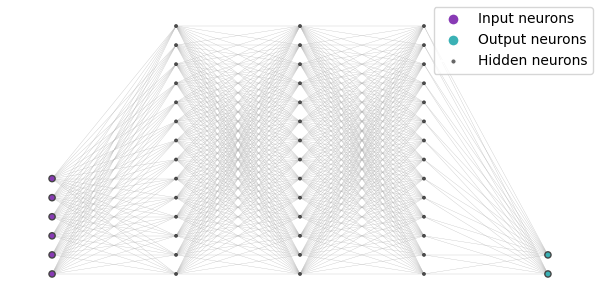
\includegraphics[scale=0.58]{figs/ann_architecture}
	\begin{center}
		\small Figure 1. Example ANN architecture (baseline)
	\end{center}
	
	\vspace{5pt}
	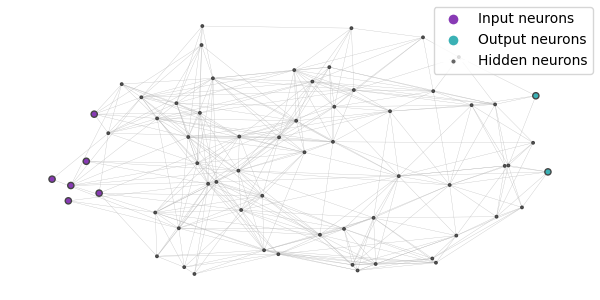
\includegraphics[scale=0.58]{figs/ant_architecture_2}
	\begin{center}
		\small Figure 2. Example ANT architecture (initialization)
	\end{center}
	
	\vspace{5pt}
	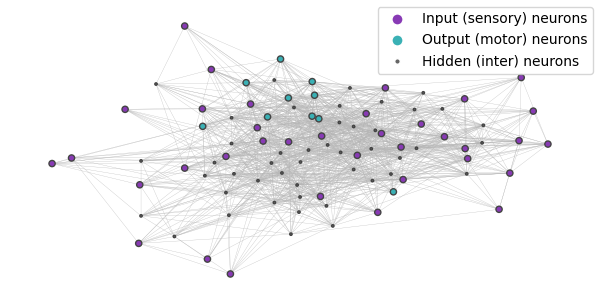
\includegraphics[scale=0.58]{figs/celegans_architecture_2.png}
	\begin{center}
		\small Figure 3. Subgraph of \textit{C. elegans} neural topology \cite{varshney2011}
	\end{center}

	This structure, while not an exact replica of neural topology, when combined with the genetic algorithm (see \textbf{3.3}) provides a superset of the hypothesis class which can mimic the neural circuit structures found in biological networks by forming recurrent, potentially cyclic dynamic relationships between neurons.
	
	\subsection{Update and Learning Mechanism} 
	
	Unlike conventional artificial neural networks, ANT, like its biological counterpart, behaves dynamically across time. At each timestep $t$ a set of inputs $\mathcal{X}$ of length $\ell$ are distributed to each of $\ell$ input neurons (where $\ell$ is defined at initialization). Then, simultaneously each neuron $v_i$ computes $y_i = x_iw_i + b_i$ and applies $\sigma_i$ on $y_i$, where $x_i$ at time $t$ is the outputs of inbound neurons at $t - 1$, and distributes each vector component of $y_i$ through corresponding outbound edges. The output $\hat{\mathcal{Y}}$ of the network is then the concatenated single-dimensional outputs of each output neuron.
	
	Recent advances in the study of biological neurons reveal a complex learning mechanism within individual dendritic connections and synaptic clefts, as well as the known properties of the soma \cite{dendrite1} \cite{dendrite2} \cite{dendrite3} \cite{dendrite4}. With this, we model individual neurons as multiple perceptron relationships between inputs and outputs, rather than a more conventional single perceptron approach. Practically, weight matrix then becomes two-dimensional with a corresponding 1-dimensional bias vector.
	
	Because ANT is designed to behave dynamically and learn continually, the gradient computation must be compatible with online updates as well. Typically, for a loss function $L$, proceeds by passing backward the product of an upstream jacobian with locally computed input gradients to compute a local partial derivative with respect to loss
	
	$$\frac{\partial L}{\partial w_i} = \frac{\partial L}{\partial x_m} \cdot \frac{\partial x_m}{\partial x_l} \dots \frac{\partial x_k}{\partial x_j} \cdot \frac{\partial x_j}{\partial w_i},$$
	
	 in a network where $v_i \rightarrow v_j \rightarrow \dots \rightarrow v_l \rightarrow v_m$ However, a conventional backpropagation approach from ANNs mandates an acyclic graph to eliminate a circular dependency causing infinite gradient chains, preventing precomputing backpropagation chains. Therefore, gradients must be dynamically passed backward in a similar manner to forward propagation, where only one gradient passing ``step'' occurs at each $t$. This links the dependence of each partial gradient component of the chain to the timestep at which it was computed, barring cancellation in the expansion for an arbitrary $L, w_i$:
	 
	 \begin{equation*}
	 	\begin{split}
	 		\frac{\partial L}{\partial w_{i_{t + k}}} & \neq \frac{\partial L}{\partial x_{m_t}} \cdot \frac{\partial x_{m_{t + 1}}}{\partial x_{l_{t + 1}}} \dots \frac{\partial x_{k_{t + k - 1}}}{\partial x_{j_{t + k - 1}}} \cdot \frac{\partial x_{j_{t + k}}}{\partial w_{i_{t + k}}}
	 	\end{split}
	 \end{equation*}
	 
	 To mathematically satisfy this approach, we can closely approximate the gradient chain by instead only episodically updating network weights at relatively distant time intervals, removing the weight parameter's dependence on time. Then, for any adjacent neurons $i \rightarrow j$ passing gradients backward at $t, t + 1$, respectively,
	 
	 \begin{equation*}
	 	\begin{split}
	 		\frac{\partial x_{k_t}}{\partial x_{j_t}} \cdot \frac{\partial x_{j_{t + 1}}}{\partial x_{i_{t + 1}}} & = \frac{\partial \sigma_j(y_{j_{t}})}{\partial y_{j_{t}}} \cdot \frac{\partial y_{j_{t}}}{ \partial x_{j_{t}}} \cdot \frac{\partial \sigma_i(y_{i_{t + 1}})}{\partial y_{i_{t + 1}}} \cdot \frac{\partial y_{i_{t + 1}}}{ \partial x_{i_{t+1}}} \\
	 		& = \frac{\partial \sigma_j(y_{j_{t}})}{\partial y_{j_{t}}} \cdot w_{j_{t}} \cdot \frac{\partial \sigma_i(y_{i_{t + 1}})}{\partial y_{i_{t + 1}}} \cdot w_{i_{t + 1}} \\
	 		& = \frac{\partial \sigma_j(y_{j_{t}})}{\partial y_{j_{t}}} \cdot w_{j} \cdot \frac{\partial \sigma_i(y_{i_{t + 1}})}{\partial y_{i_{t + 1}}} \cdot w_{i}
	 	\end{split}
	 \end{equation*}
	 
	 \noindent which, with an activation function that's near linear\footnote{An example of such an activation is $a_n(x) = n\tanh(\frac{x}{n})$, where $a_n(x) = x$ as $n \rightarrow \infty$} across most of $\mathbb{R}$, approximates
	 
	 \begin{equation*}
	 	\begin{split}
	 		\frac{\partial \sigma_j(y_{j_{t}})}{\partial y_{j_{t}}} \cdot w_{j} \cdot \frac{\partial \sigma_i(y_{i_{t + 1}})}{\partial y_{i_{t + 1}}} \cdot w_{i} & \approx 1 \cdot w_{j} \cdot 1 \cdot w_{i} \\
	 		& = \frac{\partial x_{k}}{\partial x_{j}} \cdot \frac{\partial x_{j}}{\partial x_{i}} \\
	 		& = \frac{\partial x_{k}}{\partial x_{i}},
	 	\end{split}
	 \end{equation*}
	 
	 \noindent as desired. Applying this principle to the full gradient computation, ANT approximates a dynamically learning algorithm, similar to biological networks. We use the RMSProp \cite{hinton2018} as a parameter optimizer for this work.
	 
	 
	 
	 \subsection{Evolution}
	 
	 To further emulate its biological counterpart, ANT also performs a genetic search over the hyperparameter space. Specifically, ANT modifies the connectivity and neuron count of the network. Specifically, for each mutation and with uniform $E \sim $ Unif$(0, 1)$, edges are added with probability $E \leq p \cdot \frac{2e}{n(n - 1)}$ and removed with probability $E \leq p_e \cdot \frac{n(n - 1) - 2e}{n(n - 1)}$, where $e, n$ are the current number of edges and neurons, respectively, and $p_e$ is a parameter. The number of new neurons is defined by $N \sim $ Pois$(p_n)$ with hyperparameter $p_n$.\footnote{We have not implemented neuron pruning, but this could also be included as a random variable or based on activity} The evolution of ANT thus allows for larger and more complex networks to form. The ability of the genetic algorithm to change the topology of ANT enables selectively faster information travel between areas of the network where a locally connected network would otherwise require several timesteps to propagate information. This selective minimization of the degrees of separation between distal vertices is important for the learning speed of the at-large network, quick reactionary mechanisms, and other properties of biological circuits \cite{ananth2009} \cite{menzel2001}.
	 
	 \vspace{5pt}
	\begin{center}
	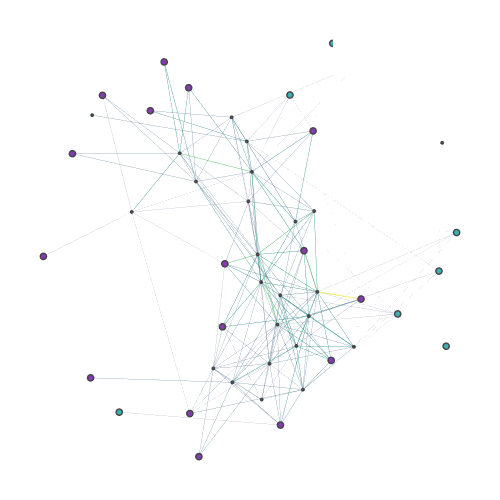
\includegraphics[scale=0.23]{figs/evolution-6}
	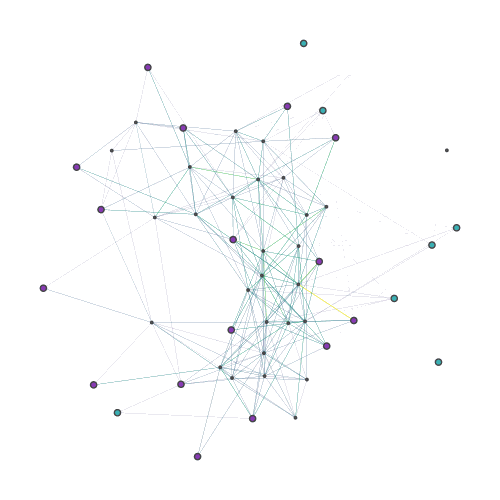
\includegraphics[scale=0.23]{figs/evolution-10}
	
	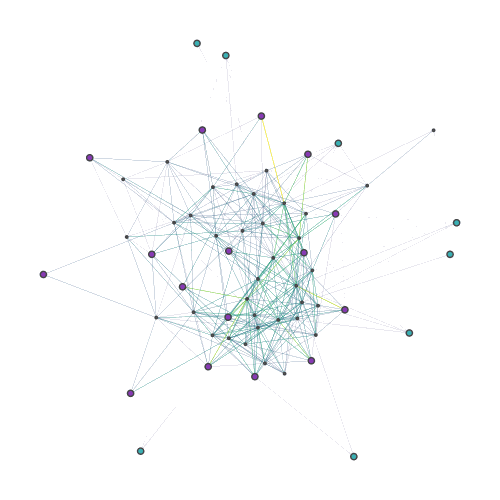
\includegraphics[scale=0.23]{figs/evolution-18}
	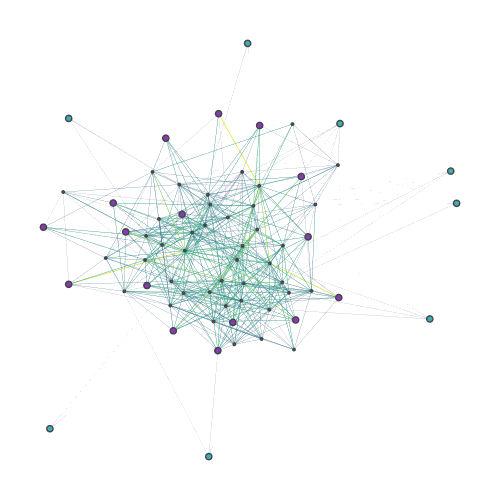
\includegraphics[scale=0.23]{figs/evolution-26}
	
		{\small Figure 4. Evolution of a small ANT}
	
	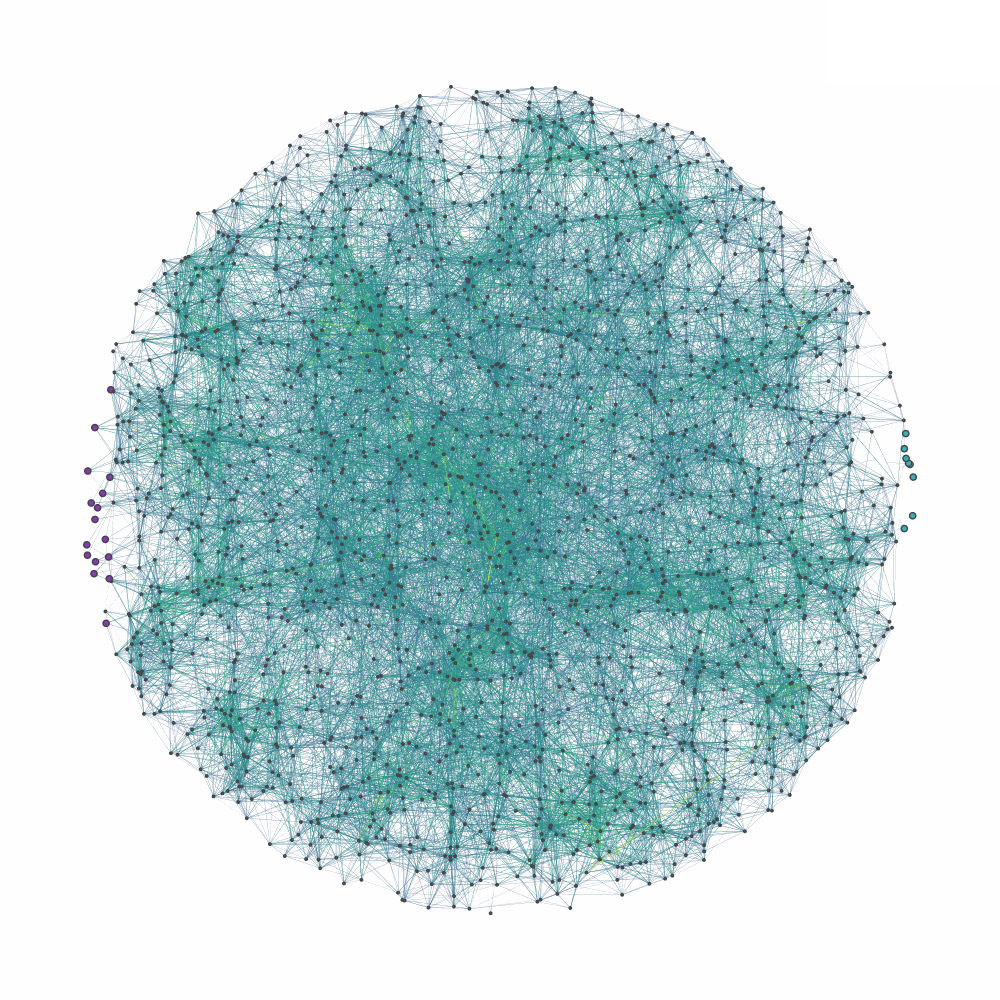
\includegraphics[scale=0.15]{figs/evolution-large}
	
	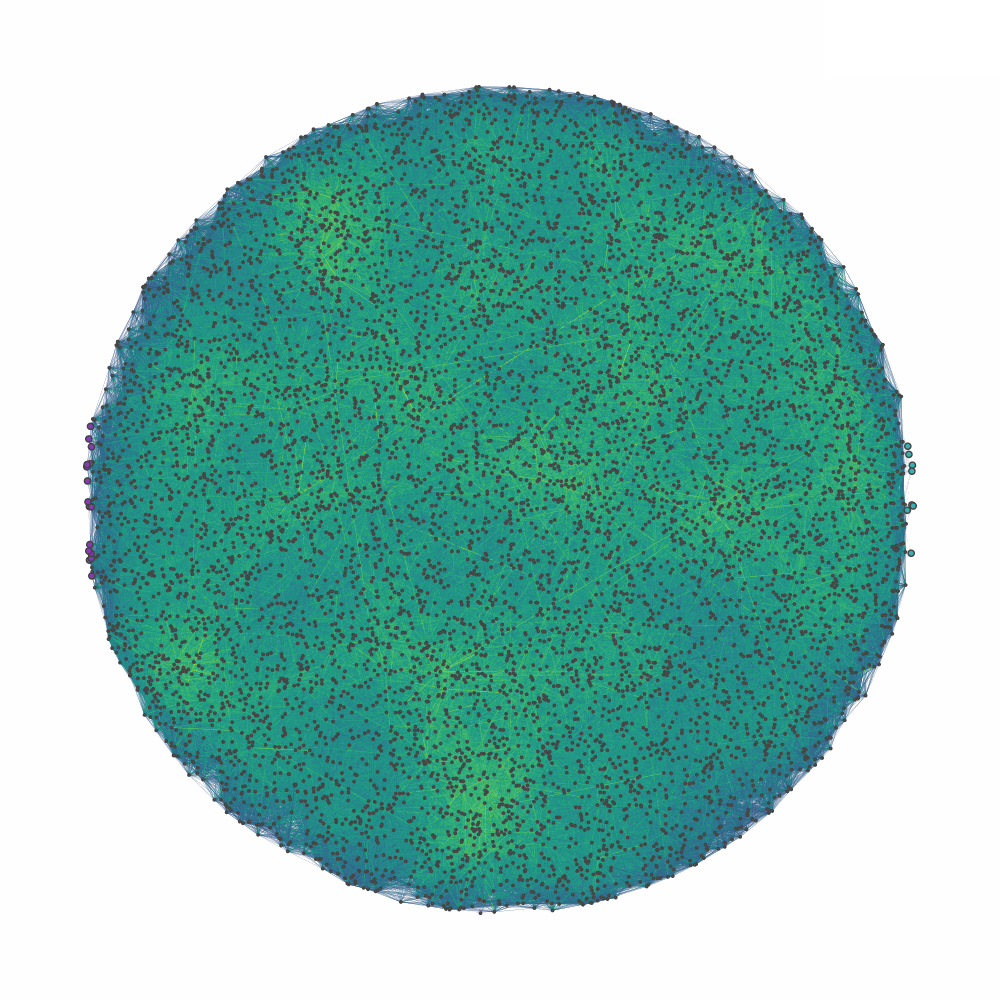
\includegraphics[scale=0.19]{figs/evolution_huge}
	
		{\small Figure 5. Evolution of a large ANT\footnote{Activity is depicted on the ``viridis" color gradient--purple is low, green/yellow is high}}
	\end{center}
	
	\subsection{Reinforcement Learning}
	
	Due to the dynamic nature of ANT coupled with the objective of pursuing generalized intelligence, we use reinforcement learning (RL) as a medium through which to compare our results to ANNs.
	
	ANT computes actions unconventionally compared to most other DQN or deep policy methods. Instead of mandating exploration with a user- or agent-controlled hyperparameter, we found exploration emergent from the dynamic structure of ANT. Intuitively, due to the variability of the input space, ANT cannot overfit in a traditional sense by forming explicit input-output mappings. In other machine learning settings this is a challenge, but in RL this leads to implicit exploration during the continual evolution of the internal state. Therefore, actions are simply determined as an argmax over the logit outputs of the network.
	
	We also use the REINFORCE (REward Increment = Nonnegative Factor × Offset Reinforcement × Characteristic Eligibility) \cite{williams1992} policy gradient method used widely across reinforcement learning. We apply REINFORCE in a semi-online setting. As described before, gradient computation must occur in real time. To comply with this constraint, we accumulate gradient-reward pairs for $T$ timesteps before applying REINFORCE to compute a gradient for the policy:
	
	\[\sum_{t=0}^{T} \left[\nabla_{\theta} \log \pi_{\theta}(a_t|s_t) \cdot \sum_{k=t}^{T} \gamma^{k-t} \cdot r_k \right]\]
	
	\medskip \noindent with discount factor $\gamma$ at each $T$ interval where $T >> 1$.

	\subsection{Experimental Setup}
	
	Our experiments are predicated on assessing ANT's ability to converge both more quickly and adaptively compared to its ANN counterpart. To assess this in a fundamental sense, we use 
	
	For comparison, we design an analogous ANN with similar mutation parameters, but only within its layered structure. For reinforcement learning, we use three discrete action-space Gym\footnote{an open-source Python library originally developed by OpenAI and now maintained by the Farama Foundation.} environments: Cartpole, Acrobot, and Lunar Lander. Cartpole is a balancing game where an agent must slide a cart to maintain the upright position of a pole. Acrobot requires an agent to apply appropriate force to a double pendulum to swing the bottom node over a certain height, and Lunar Lander requires an agent to land a lunar module with 3 thrusters on terrain.
	
	\begin{center}
		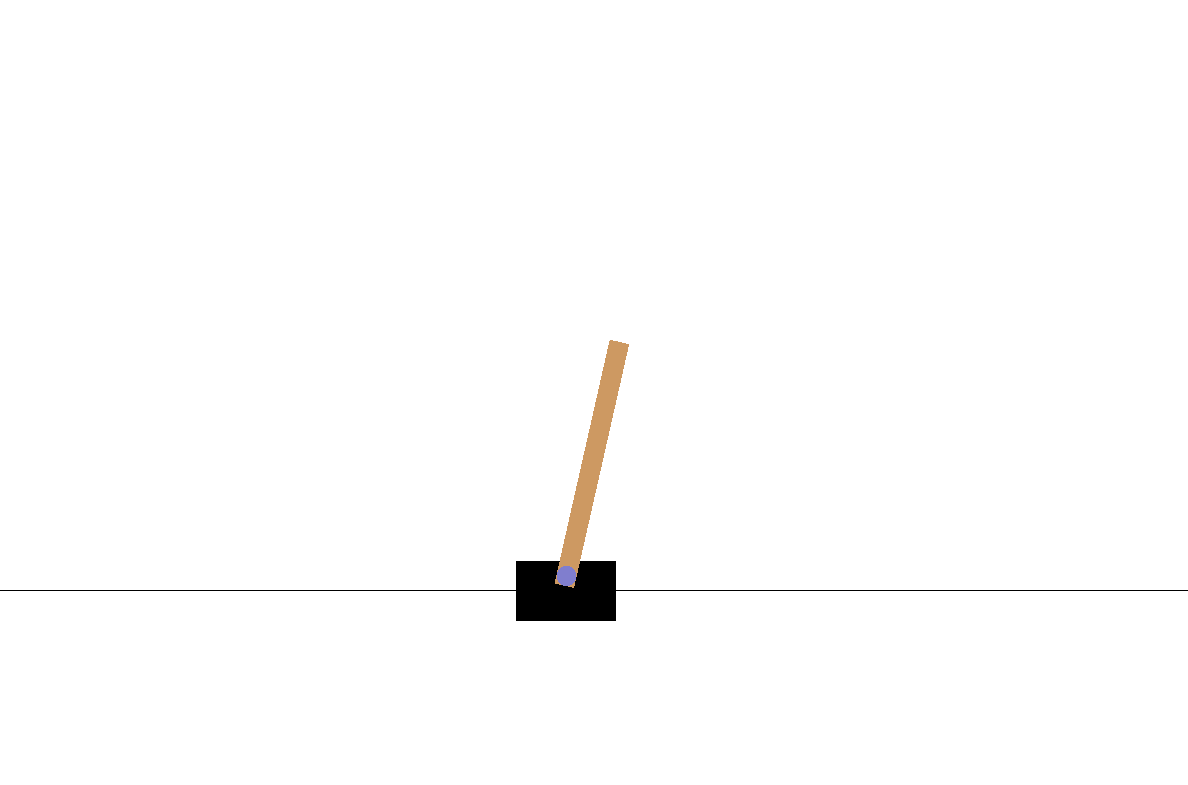
\includegraphics[scale=0.08]{figs/cartpole.png}
		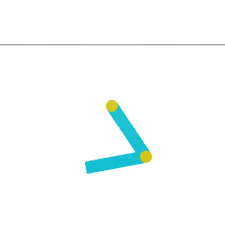
\includegraphics[scale=0.26]{figs/acrobot.png}
		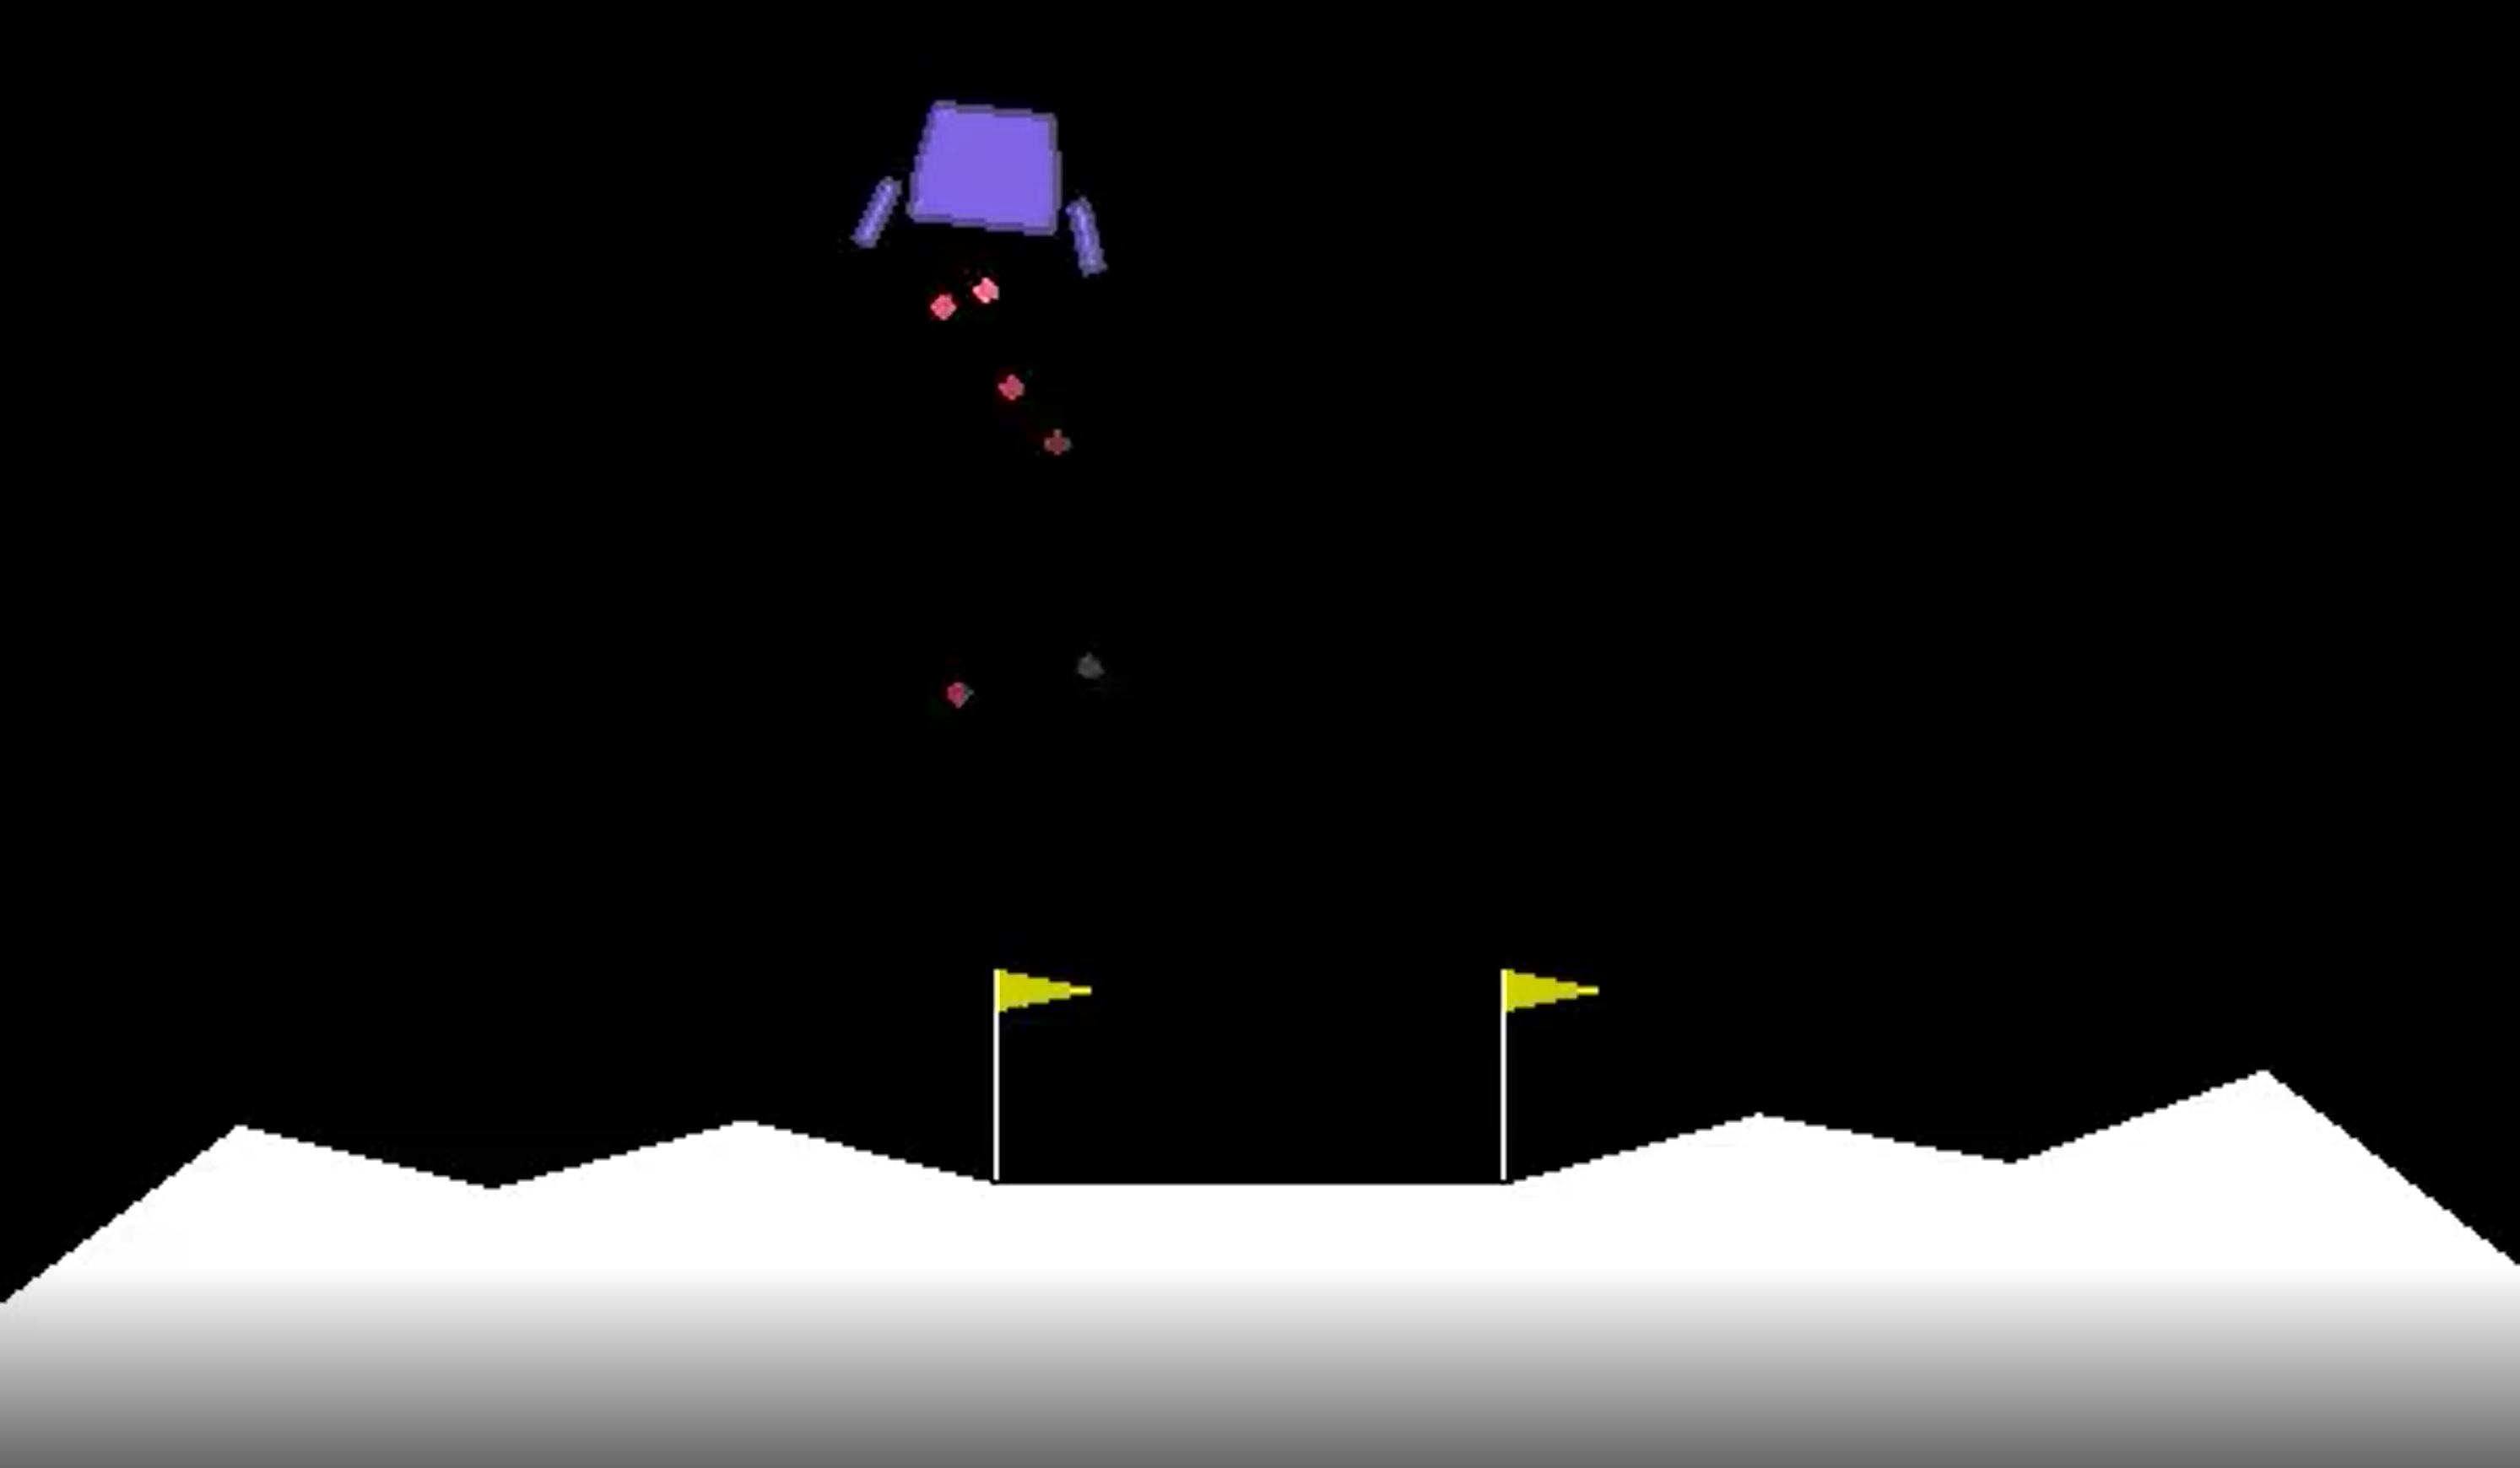
\includegraphics[scale=0.075]{figs/lunarlander.png}
		
		\footnotesize Figure 6. Cartpole (left), Acrobot (middle), Lunar Lander (right)	
	\end{center}

	
	We complement these environments with the Context Adaptive Reinforcement Library (CARL) \cite{benjamins2023}, a suite of analogously designed environments which float different physics properties to evaluate the generalizability of RL models, positing that if RL models are able to more quickly and reliably converge to high-reward solutions in environments which have object properties that vary, then they are more adaptable. While imperfect for investigating the capacity for ANT to achieve a general intelligence, at the scale of only a few dozen neurons we rationalize that a positive result in adaptability could translate to more complex reasoning behavior for larger-scale, more sophisticated topologies.
	
	To train parameter efficiency, we create a ``small'' version of each model with 36 neurons and roughly $\sim450$ trainable parameters and a ``large'' version of each with 66 neurons and $\sim$1170 trainable parameters. In both cases, the ANN is structured as an MLP with 2 hidden layers while the ANT has a connectivity parameter $p_e$ of 1.4, each with input and output sizes equal to the observation and action spaces of each respective environment.
	
	We first compare the efficacy of an isolated gradient descent approach for training in each environment. For each experiment, we run 1000 epochs of the environment with reporting the best result across a search of 20 unique learning rate parameters.
	
	\begin{center}
		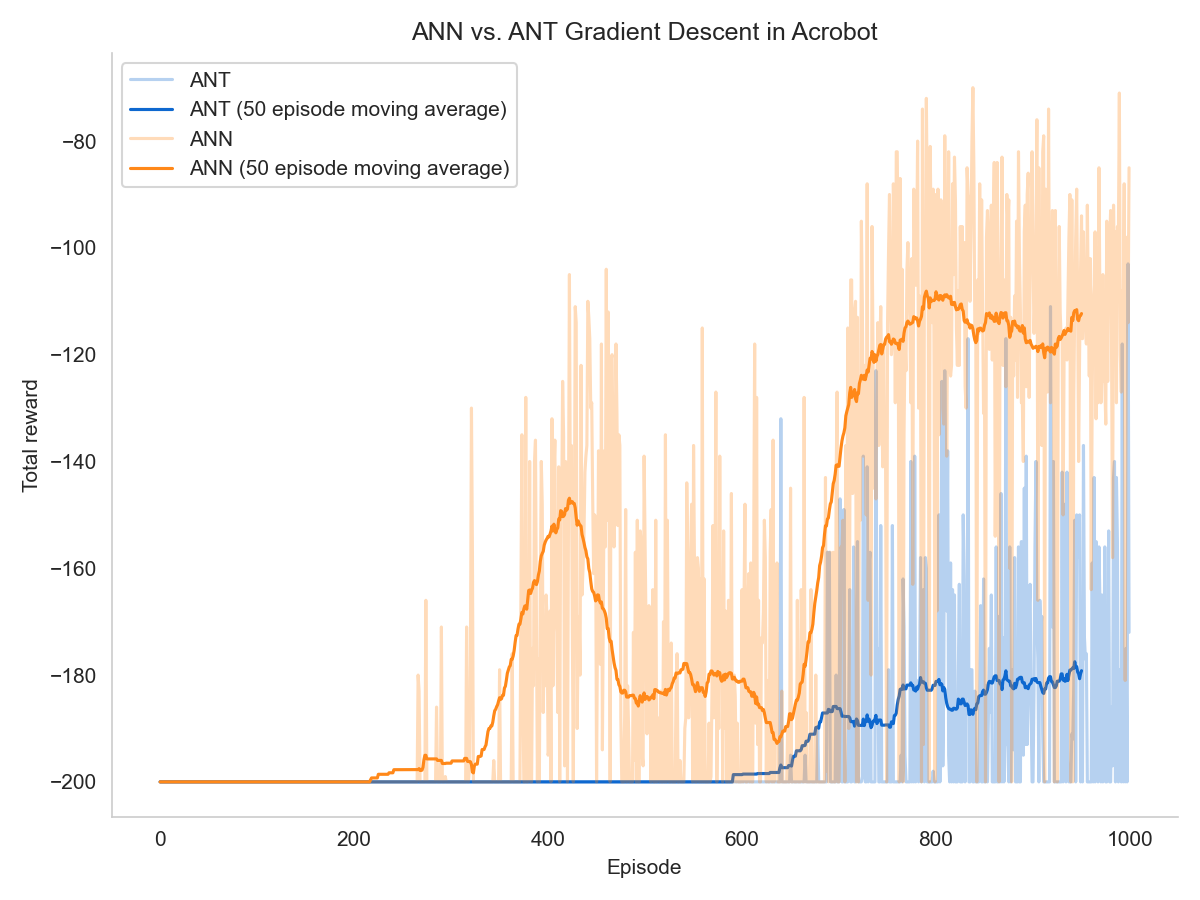
\includegraphics[scale=0.22]{figs/ann_ant_acrobot.png}
		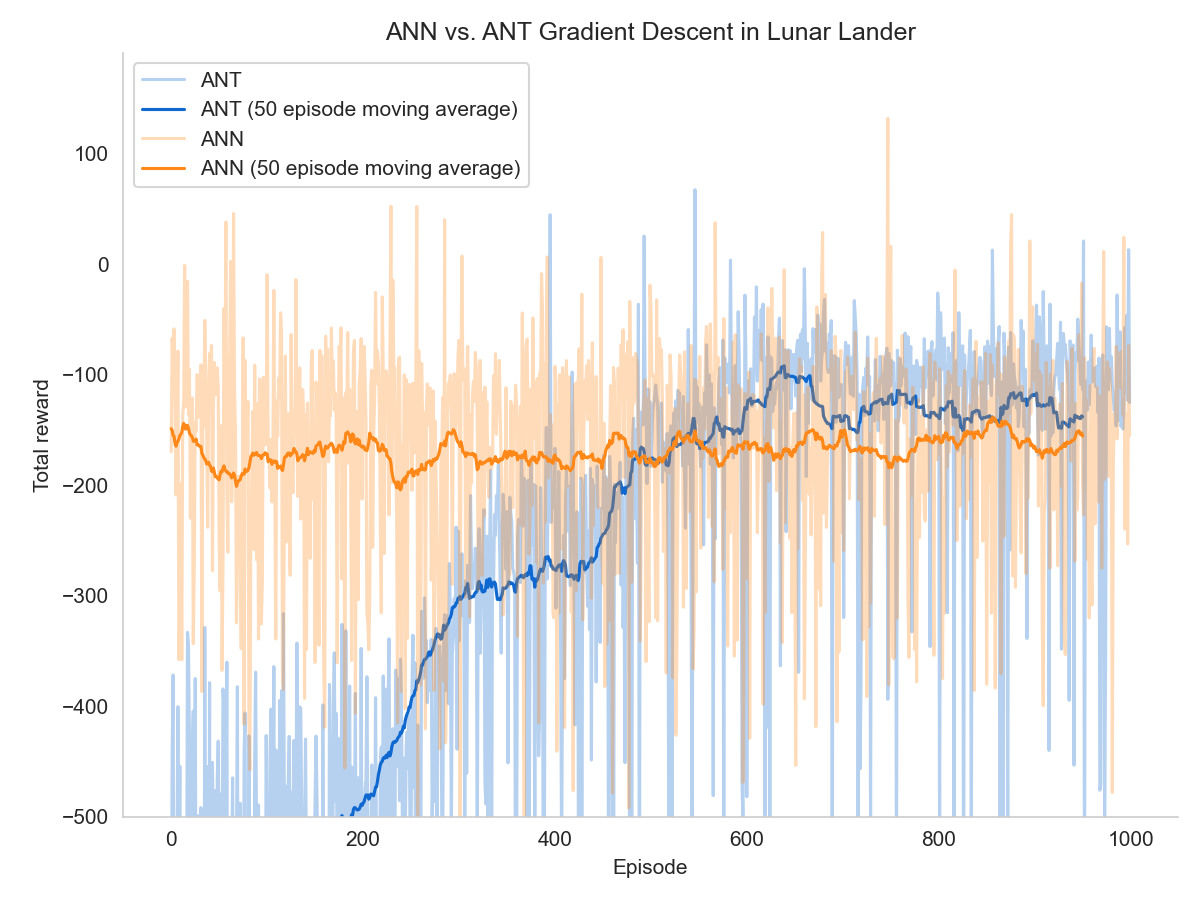
\includegraphics[scale=0.22]{figs/ann_ant_lunarlander.png}
		
		\small Figure 7. Sample ANN and ANT performance in Acrobot (left) and Lunar Lander (right) with only gradient descent
	\end{center}
	
	We run a similar experiment to test a joint gradient descent-evolutionary learning algorithm. For these experiments, we fix the two initial network structures as in SGD. For 20 evolutionary episodes, we first collect the top $k = 5$ networks from the previous episode, perform perturbations with a neuron addition rate regulated by $N \sim $ Pois($0.5$), an edge mutation rate with $p_e = 0.05$, and a weight perturbation with $W \sim \{\mathcal{N}(0, 1 \times 10^{-4})\}_{i = 1}^{e}$ for a network with $e$ edges.\footnote{We maintain the same graph properties for the ANN. We only add vertices and edges to layers, as opposed to randomly connecting each to the existing graph as done in ANT evolution.} Each network is then trained for 100 episodes, after which an average reward is computed to determine the top-$k$. Below is an illustration of the best performing evolutionary path for the ANN and ANT in each environment, as well as close-performing neighbors.
	
	\begin{center}
		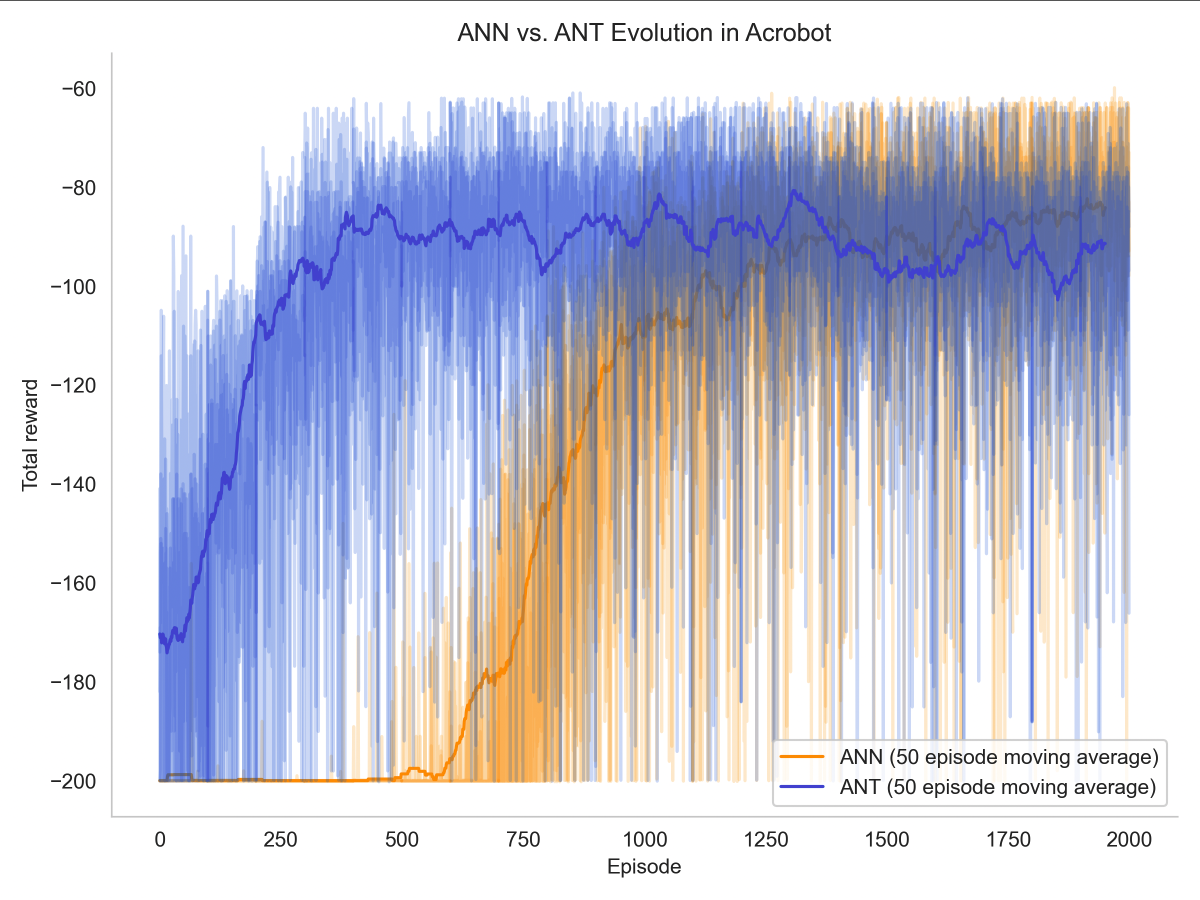
\includegraphics[scale=0.1]{figs/ann_ant_acrobot_evolution.png}
		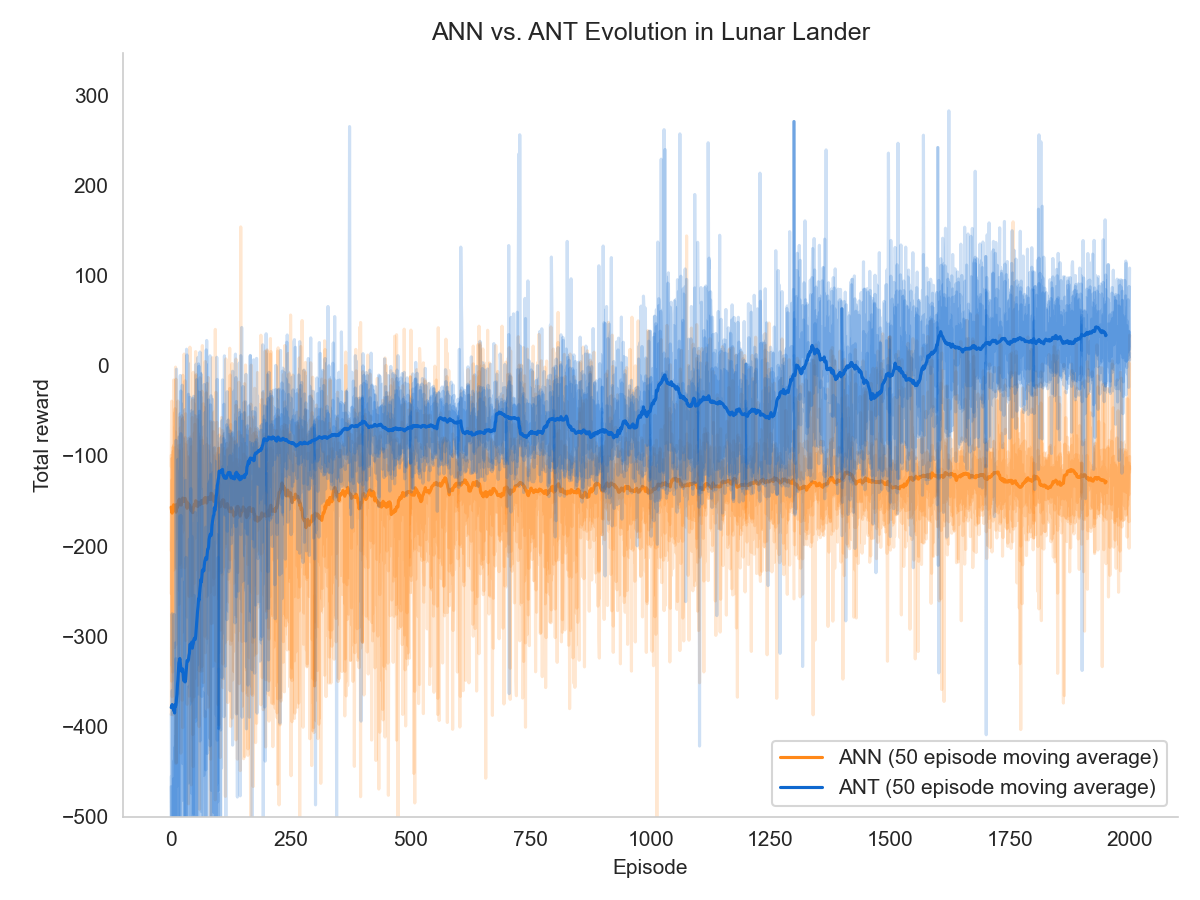
\includegraphics[scale=0.21]{figs/ann_ant_lunarlander_evolution.png}
		
		\small Figure 8. Sample ANN and ANT performance in Acrobot (left) and Lunar Lander (right) with evolution and gradient descent
	\end{center}
	
	\subsection{Robotics}
	
	Operating from the Reward is Enough hypothesis, which posits that all aspects of intelligence subserve reward maximization by an agent acting in its environment, ANT can behave analogously to animals through policy optimization [10]. Conversely, this implies that our proposed agent can develop multiple aspects of intelligent behavior given a simple design of such a reward function.
	
	We developed both a virtual and physical agent with analogous environmental setups, where an agent navigates a 2D environment populated with obstacles and food. Upon reaching a food object, the agent receives a reward. The food-finding reward is intended to incentivize the agent to efficiently navigate its environment to move toward the food object. In generalizing the environment to a small sensor-based observation space, the model forgoes assumptions about its environment and embraces continual learning. This further enables the agent to adapt to a non-stationary environment. At each timestep, the agent makes a partial observation of its state, formulated as a 2-dimensional feature vector encoding the distance to the nearest object or obstacle in front of the agent as well as a boolean value indicating if food is present in the agent’s field of vision. The agent can take 5 possible actions at each timestep: wait, rotate right, rotate left, move forward, or move backward.

	For the physical agent, the observation space is observed using an ultrasonic sensor and Pixy2 camera. The ultrasonic sensor tracks the distance measurement to objects in front of the agent, and the Pixy2 has built-in object detection functionality to determine if ‘food’ is present in its field of vision. The agent executes actions using two DC motors controlled with an L298N motor controller (Figure XB). After training ANT on the virtual environment, the trained network can be uploaded onto the physical agent to operate the agent and continue to learn. We hypothesize that a sophisticated embodiment of ANT should exhibit sophisticated, animal-like behavior.
	
	\section{Results}
	
	We aim to demonstrate that, while conventional artificial neural networks are unable to converge quickly for small parameter counts, ANT can converge both quickly and robustly with high sample and parameter efficiency. We will first represent a sample learning trajectory for each experiment, then establish the rate of convergence.
	
	\subsection{Baseline Reinforcement Learning}
	
	With ANN-small and ANT-small as networks defined with 36 neurons neurons and 66 neurons, respectively, we take the mean final reward over 100 different training runs with each model type.
	
	\begin{center}
	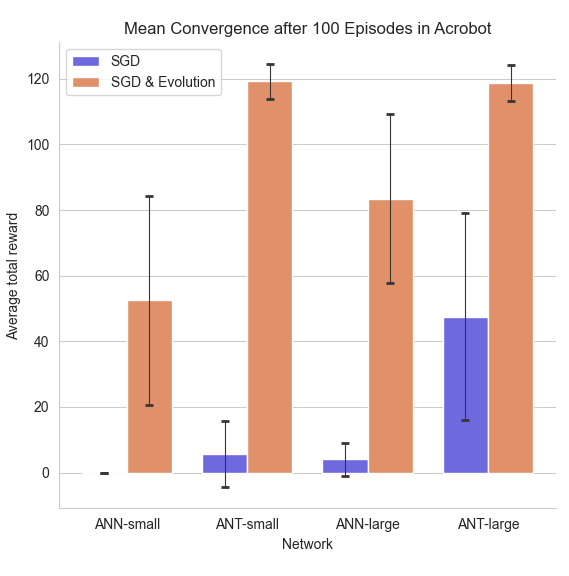
\includegraphics[scale=0.6]{figs/acrobot_convergence_reshaped.png}
	\small Figure 9. ANN and ANT 100 episode convergence for Acrobot
	\end{center}
	
	In Figure 9, this experiment is run on Acrobot with an expected optimal total reward of approximately 140 for a 200-timestep game,\footnote{Acrobot penalizes each non-successful step with a reward of $-1$, so for illustrative clarity, we report the reward as 200 $+$ total reward, where each episode is 200 timesteps, so as to avoid strictly negative rewards. We do not do this for LunarLander.} with a sufficiently positive result exceeding 100 and a negative result (unable to complete the task) as 0. For models trained only on gradient descent, ANT outperforms both the small and large ANNs significantly, demonstrating an ability to complete the game at remarkably low parameter counts for a quick training cycle and even better convergence for the large model. Given a genetic algorithm with SGD, ANT converges to a near-optimal solution uniformly for both the small and large model, significantly outpacing their ANN counterparts.
	
	\begin{center}
	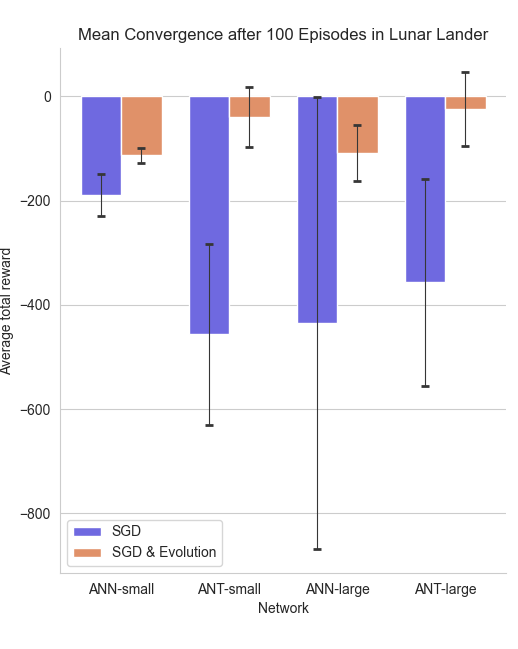
\includegraphics[scale=0.6]{figs/lunarlander_convergence_resize.png}
	\small Figure 10. ANN and ANT 100 episode convergence for Acrobot
	\end{center}
	
	For a more sophisticated game like Lunar Lander with a 50\% larger action and observation space on a more complex 2D game, we see that while ANT-small and each of the larger models fail to converge to an optimal solution (above 0) in 100 timesteps, ANT again routinely approaches this reward using the combined genetic-gradient descent algorithm, with the $1\sigma$ error bar in for both the small and large model indicating that around 30-40\% of the trained models achieved an optimal solution.

	
	\subsection{CARL}
	
	\subsection{Robot Performance}
	
	Despite some successes in simulation, the translation to a physical agent failed due to the narrow observation space and discrepancies between the simulated and real-world environments.
 
For the physical agent, the ultrasonic sensor was prone to inconsistent distance measurements, and the computer vision algorithm frequently failed to detect the food or misidentified other objects as food. These inaccuracies led to suboptimal decision-making and performance failures. Our attempts to rectify these issues through a hard-coded algorithm to locate food were unsuccessful, with a success rate of 20\%. The failure of a hard-coded algorithm underscores that the performance failures are, in large part, due to limitations of the physical agent itself rather than the underlying network. This highlights the need for an expanded observation space, which could include integrating multiple sensors to take distance measurements at various angles.

Similarly, the ANT network was first trained in a controlled virtual environment, which does not adequately capture the complex dynamics of the physical world. Sensor inconsistencies, variations in motor functions, and dynamic environment elements were not modeled in the simulation and warrant a more intricate simulation environment. Incorporating Partially Observable Markov Decision Processes (POMDPs) could be beneficial in modeling the uncertainties and variabilities inherent in real-world interactions, leading to a more robust and adaptable agent.
	
	\subsection{Performance and Scalability}
	
	Due to the dynamic nature of ANT, the complexity of the update procedure runs linearly with respect to the number of neurons while suboperations within neurons require a linear compute time with respect to the number of connections, leading to a generally quadratic overall compute time. However, ANT is highly parallelizable, with each neuron operation occurring independently of other neurons and with genetic iterations that also run independently of other trials. 
	
	\begin{center}
		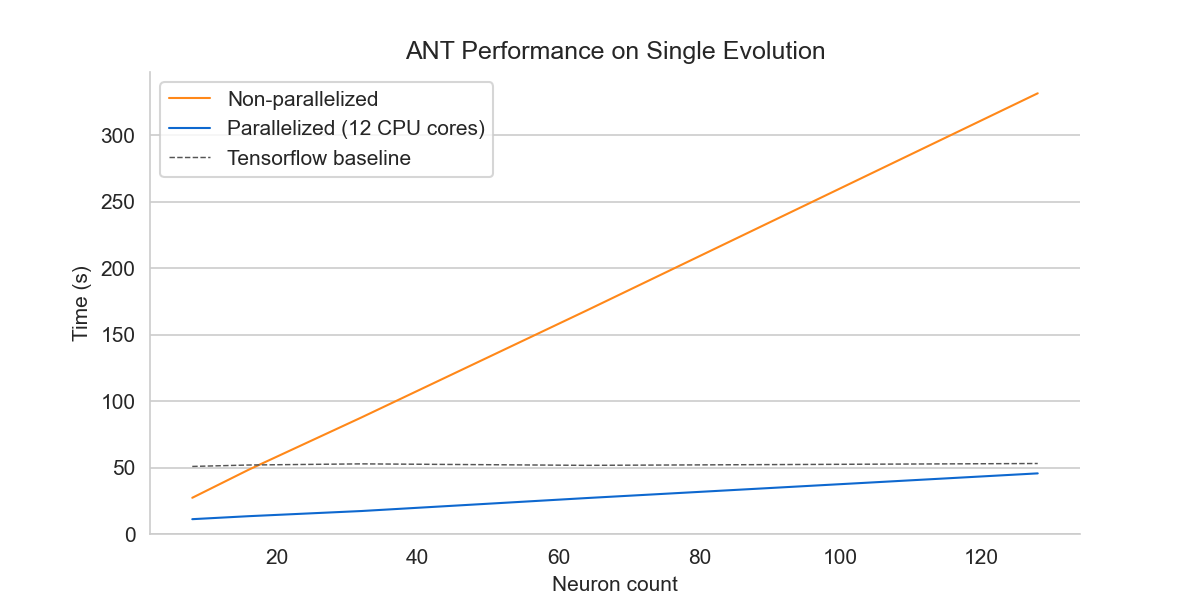
\includegraphics[scale=0.47]{figs/ant_performance_2.png}
		\small Figure 12. Speed of ANT with connectivity $\frac{1}{\sqrt{n}}$
	\end{center}

	
	ANT is currently constructed with Python which has a Global Interpreter Lock (GIL) preventing process threading, so we anticipate that a raw C/C++ implementation with threaded neuron operations would be even more computationally advantageous.
	
	As opposed to the few large matrix compositions involved in ANN forward and backward propagation, most of the computations in ANT, while parallelizable, involve many relatively small matrix operations. This imposes a necessary bound on the compute speed of ANT relative to conventional networks--where ANNs can use inbuilt matrix composition optimizations common in today's Graphics Processing Units (GPUs), these improvements aren't reflected to nearly the same degree on smaller compositions. 
	
	However, ANT's computation is invariant of a notion of network ``depth.'' Where ANNs require the sequential computation of outputs and gradient depthwise, ANT can compute all gradients in parallel. When shifting the baseline to instead make deeper instead of wider networks, reducing the optimizability of its gradient calculation, ANT becomes distinctly more advantageous:
	
	\begin{center}
		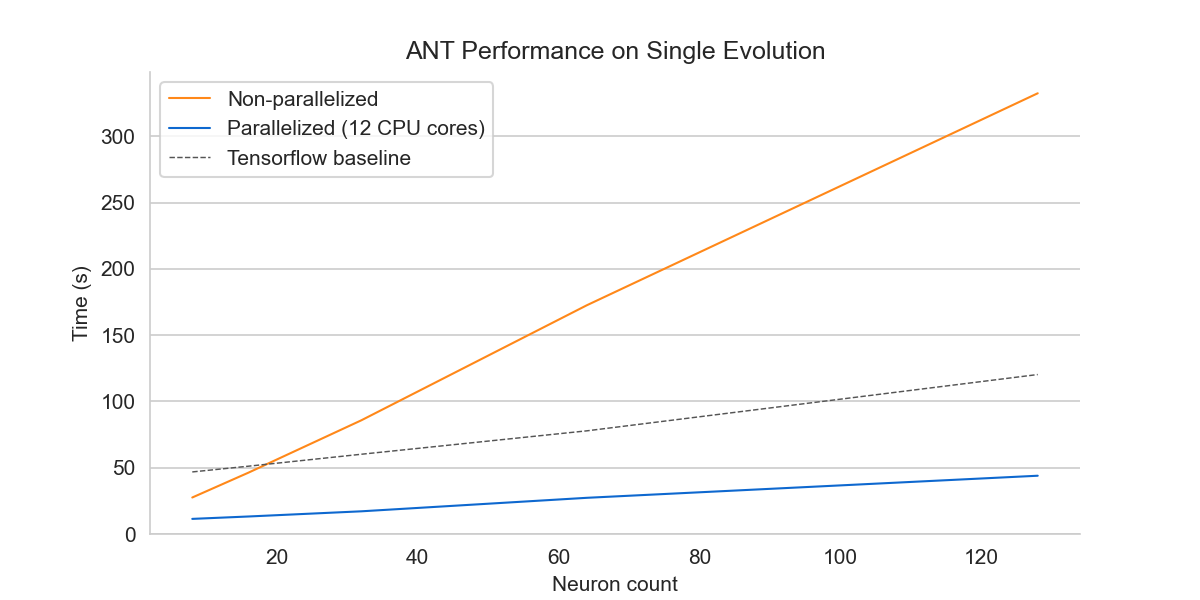
\includegraphics[scale=0.47]{figs/ant_performance_3.png}
		\small Figure 13. Speed of ANT with connectivity $\frac{1}{\sqrt{n}}$ (depthwise-expanded baseline network)
	\end{center}
	
	More experimentation with a more optimized code and better hardware is required to be conclusive on the speed of ANN compared to ANT, though it is likely that the computational tradeoff is problem-specific.
	
	\section{Summary and Conclusion}
	
	\subsection{Limitations}
	
	There are several limitations of the ANT formulation which complicate its use in most machine learning contexts. Because it is a dynamic network, ANT is not known to be capable of making distinct input-output functional pairings as in the context of supervised learning. In fact, in all settings which involve sharp discontinuities, heavy discretization of input, or non-temporal input, ANT's formulation seems to preclude it from use.\footnote{It is possible that supervised tasks would work if presented in an RL-like setting.}
	
	Further, not studied heavily in this paper is the sensitivity of ANT to initial conditions. As desired network complexity increases, the hyperparameter space grows exponentially as the total number of possible graph structures itself increases at a rate of $2^n$ where, as we have seen anecdotally, different graph constructions can yield significantly different convergence times. In most cases for particular RL settings, ANT would fail to converge completely given some graph initialization via stochastic gradient descent. This requires the use of a genetic algorithm that, though optimizable, is a much more brute-force approach toward searching for viable network structures and may not be computationally feasible for large parameter spaces.
	
	\subsection{Future Work}
	ANT is a novel neural network formulation which we believe shows significant promise for applications in RL.
	
	The properties of ANT remain largely unstudied. Although we have investigated small-scale applications of ANT in RL studies in this paper, scaled RL applications and alternative machine learning applications are unknown. It is possible that scaling ANT is computationally difficult, however if the results at small scales indicate a similar convergence speeds for higher parameter counts then it would be worthwhile, especially if transfer learning were possible. Alternatively, like many dynamic networks, the convergence properties of ANT may be revealing in studying how biological neural networks may retain information, such as the memory-retention properties of Hopfield networks \cite{hopfield1977}.
	
	We also haven't investigated the graphs created by ANT's evolutionary algorithm. It is likely that they or their internal dynamics have emergent characteristics that could inform future development of ANT or other learning dynamic networks.
	
	The goal of an artificial neural topology is to emulate the reasoning behavior of prefrontal cortices from large animals. We believe that ANT is a step toward a generally reasoning agent, and in an embodied context paired through a conjoined latent space with even task specific computer vision, audio, and sensorimotor models could serve as the final building block to the reintegration of artificial intelligence through true task-generalizability.

\begin{thebibliography}{11}

\bibitem{vaswani2017} Vaswani, Ashish, et al. "Attention is all you need." Advances in neural information processing systems 30 (2017). 

\bibitem{ngaim2011} Ngiam, Jiquan, et al. "Multimodal deep learning." Proceedings of the 28th international conference on machine learning (ICML-11). 2011.

\bibitem{taloni2023} Taloni, Andrea, et al. "Comparative performance of humans versus GPT-4.0 and GPT-3.5 in the self-assessment program of American Academy of Ophthalmology." Scientific Reports 13.1 (2023): 18562.

\bibitem{sonoko2024} Sonko, Sedat, et al. "A critical review towards artificial general intelligence: Challenges, ethical considerations, and the path forward." World Journal of Advanced Research and Reviews 21.3 (2024): 1262-1268.

\bibitem{li2023} Li, Yingbo, and Yucong Duan. "The Wisdom of Artificial General Intelligence: Experiments with GPT-4 for DIKWP." arXiv preprint (2023).

\bibitem{goertzel2014} Goertzel, Ben. "Artificial General Intelligence: Concept, State of the Art, and Future Prospects" Journal of Artificial General Intelligence, vol.5, no.1, 2014, pp.1-48. https://doi.org/10.2478/jagi-2014-0001

\bibitem{azevedo2009}
Azevedo FAC, Carvalho LRB, Grinberg LT, Farfel JM, Ferretti REL, Leite REP, et al. 
Equal numbers of neuronal and nonneuronal cells make the human brain an isometrically scaled-up primate brain. 
\textit{J Comp Neurol}. 2009 Apr;513(5):532-41. 
doi:10.1002/cne.21974. PMID:19226510. S2CID:5200449.

\bibitem{ananth2009}
Ananthanarayanan R, Esser SK, Simon HD, Modha DS. 
The cat is out of the bag: cortical simulations with 109 neurons, 1013 synapses. 
In: \textit{Proc Conf High Perform Comput Netw Storage Anal - SC '09}; 2009. p. 1-12. 
doi:10.1145/1654059.1654124. ISBN: 978-1-60558-744-8.

\bibitem{claude}
Anthropic. 
Model Card for Claude 3. [Internet]. 2023. 
Available from: https://www-cdn.anthropic.com/de8ba9b01c9ab7cbabf5c33b 80b7bbc618857627/Model\_Card\_Claude\_3.pdf

\bibitem{maad2023} Mijwil Maad, Hiran Kamal, Doshi Ruchi, Dadhich Manish, Al-Mistarehi Abdel-Hameed, Bala Indu. (2023). ChatGPT and the Future of Academic Integrity in the Artificial Intelligence Era: A New Frontier. Al-Salam Journal for Engineering and Technology. 2. 116-127. 10.55145/ajest.2023.02.02.015.

\bibitem{houzel2005}
Herculano-Houzel S, Lent R. 
Isotropic fractionator: a simple, rapid method for the quantification of total cell and neuron numbers in the brain. 
\textit{J Neurosci}. 2005 Mar;25(10):2518-21. 
doi:10.1523/jneurosci.4526-04.2005. PMC 6725175. PMID: 15758160.

\bibitem{houzel2006}
Herculano-Houzel S, Mota B, Lent R. 
Cellular scaling rules for rodent brains. 
\textit{Proc Natl Acad Sci U S A}. 2006 Aug;103(32):12138-43. 
doi:10.1073/pnas.0604911103. PMC 1567708. PMID: 16880386.

\bibitem{menzel2001}
Menzel R, Giurfa M. 
Cognitive architecture of a mini-brain: the honeybee. 
\textit{Trends Cogn Sci}. 2001 Feb;5(2):62-71. 
doi:10.1016/S1364-6613(00)01601-6. PMID: 11166636.

\bibitem{reghr2012}
Regehr WG. Short-term presynaptic plasticity. Cold Spring Harb Perspect Biol. 2012 Jul 1;4(7):a005702. doi: 10.1101/cshperspect.a005702. PMID: 22751149; PMCID: PMC3385958.

\bibitem{basset2006}
Bassett, D. S., \& Bullmore, E. (2006). Small-world brain networks. The Neuroscientist, 12(6), 512-523.

\bibitem{varshney2011}
Varshney, Lav \& Chen, Beth \& Paniagua, Eric \& Hall, David \& Chklovskii, Dmitri. (2011). Structural Properties of the Caenorhabditis elegans Neuronal Network. PLoS computational biology. 7. e1001066. 10.1371/journal.pcbi.1001066. 

\bibitem{hinton2018}
Geoffrey Hinton, "Coursera Neural Networks for Machine Learning lecture 6", 2018.

\bibitem{herculano2005}
Herculano-Houzel S, Lent R. 
Isotropic fractionator: a simple, rapid method for the quantification of total cell and neuron numbers in the brain. 
\textit{J Neurosci}. 2005 Mar;25(10):2518-21. 
doi:10.1523/jneurosci.4526-04.2005. PMC 6725175. PMID: 15758160.

\bibitem{herculano2006}
Herculano-Houzel S, Mota B, Lent R. 
Cellular scaling rules for rodent brains. 
\textit{Proc Natl Acad Sci U S A}. 2006 Aug;103(32):12138-43. 
doi:10.1073/pnas.0604911103. PMC 1567708. PMID: 16880386.

\bibitem{benjamins2023}
Benjamins, Carolin, et al. Contextualize Me - The Case for Context in Reinforcement Learning. 2023.

\bibitem{williams1992}
Williams, R.J. Simple statistical gradient-following algorithms for connectionist reinforcement learning. Mach Learn 8, 229–256 (1992). https://doi.org/10.1007/BF00992696

\bibitem{hopfield1977}
John J. Hopfield (2007) Hopfield network. Scholarpedia, 2(5):1977.

\bibitem{dendrite1}
Polsky, A., Mel, B. W. \& Schiller, J. Computational subunits in thin dendrites of pyramidal cells. Nature Neuroscience 7, 621–627 (2004).

\bibitem{dendrite2}
Tran-Van-Minh, A. et al. Contribution of sublinear and supralinear dendritic integration to neuronal computations. Frontiers in Cellular Neuroscience 9, 67–67 (2015).

\bibitem{dendrite3}
Gidon, A. et al. Dendritic action potentials and computation in human layer 2/3 cortical neurons. Science 367, 83–87 (2020).

\bibitem{dendrite4}
London, M. \& Häusser, M. DENDRITIC COMPUTATION. Annu. Rev. Neurosci. 28, 503–532 (2005)

\bibitem{mijwil2023}
Mijwil MM, Kamal H, Doshi R, Dadhich M, Al-Mistarehi AH, Bala I. 
ChatGPT and the Future of Academic Integrity in the Artificial Intelligence Era: A New Frontier. 
\textit{Al-Salam J Eng Technol}. 2023;2:116-27. 
doi:10.55145/ajest.2023.02.02.015.





\bibitem{silver2021}
Silver, David, et al. Reward is enough. Artificial Intelligence, vol. 299, Oct. 2021, p. 103535, https://doi.org/10.1016/j.artint.2021.103535.
\end{thebibliography}

\end{multicols}

	
\end{document}